\documentclass{beamer}
\usetheme{Dresden}
\usepackage{amsmath}
\usepackage{commath}
\usepackage[backend=biber, style=numeric]{biblatex}
\usepackage[utf8]{inputenc} %Codierung der Eingabe
\usepackage[T1]{fontenc}      %Setzen in deutscher Sprache
\usepackage[ngerman]{babel}  %Korrekturpaket für neue deutsche Rechtschreibung
\usepackage[autostyle=true]{csquotes} %Setzen von Anführungszeichen
\usepackage[varg]{txfonts}  %Setzen der Schriftart
\usepackage{graphicx} %Einbinden von Graphiken
\graphicspath{{figs/}} %Setzen des Graphikpfads

\usepackage{siunitx}
\sisetup{locale=DE}


\pagenumbering{arabic}

\addtobeamertemplate{navigation symbols}{}{%
    \usebeamerfont{comic sans}%
    \usebeamercolor[black]{footline}%
    \hspace{3em}%
    \fontsize {9}{0} \selectfont
    \insertframenumber/\insertmainframenumber
}

\author{Matthias Gessinger, Frederik Theis}
\date{\today}
\title{Allgemeine Randbedingungen aus Bilddateien}
\institute{Uni Bonn, Strömungspraktikum}


\begin{document}

\begin{frame}
\maketitle
\end{frame}

\begin{frame}
    \frametitle{Das PNG-Dateiformat}
    \begin{minipage}[c]{0.48\textwidth}
        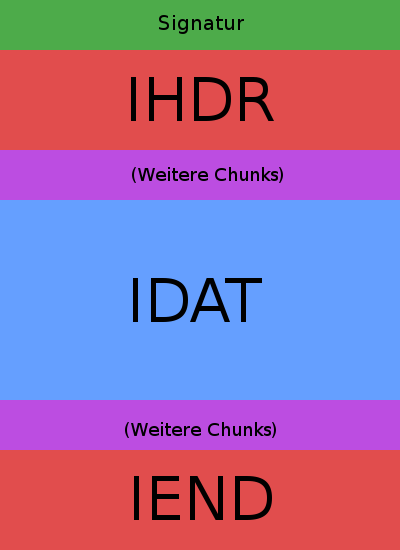
\includegraphics[height=0.8\textheight]{PNG.png}
    \end{minipage}
    \begin{minipage}[c]{0.48\textwidth}
        \begin{itemize}
            \item<1-> Signatur: \\
                  89  50  4E  47  0D  0A  1A  0A
            \item<2-> IHDR: Header-Chunk \\
                  Breite, Höhe, Farbtiefe...
            \item<3-> IDAT: Daten-Chunk \\
                  Enthält die Pixeldaten (komprimiert)
            \item<4> IEND: End-of-File-Chunk
        \end{itemize}
    \end{minipage}
\end{frame}

\begin{frame}
    \frametitle{Die png-Library}
    \begin{figure}
        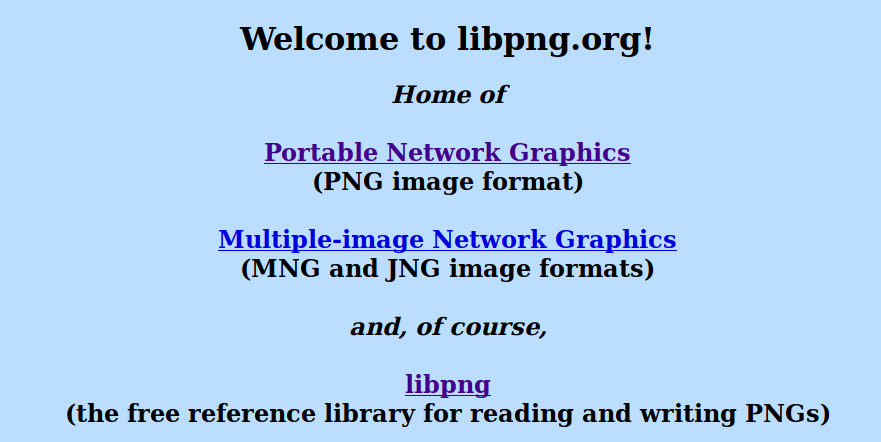
\includegraphics[width=\textwidth]{libpng.png}
        \caption{Frontseite von libpng.org}
    \end{figure}
\end{frame}

\begin{frame}
    
\includegraphics[width=0.9\textwidth]{highPixel.png}
    \hrule
    
\includegraphics[width=0.9\textwidth]{lowPixel.png}
    \hrule
\end{frame}

\end{document}
